\documentclass{acm_proc_article-sp}
\usepackage{svg}
\usepackage{listings}
\lstset{
       numberblanklines=false,
       language=make,
       tabsize=4,
       frame=single,
       keywordstyle=\color{red},
       identifierstyle= %plain identifiers for make
}
\begin{document}

\title{
BEAST TITLE TO-FILL
%\titlenote{(Does NOT produce the permission block, copyright information nor page numbering). For use with ACM\_PROC\_ARTICLE-SP.CLS. Supported by ACM.}
}
\numberofauthors{5}
\author{
\alignauthor
Yang Shichu\\
       \affaddr{School of Cyber Science and Engineering}\\
       \affaddr{Huazhong University of Science and Technology}\\
       \email{sigeryeung@gmail.com}
\alignauthor
Shu Yi\\
       \affaddr{TO-FILL}\\
       \affaddr{TO-FILL}\\
       \email{TO-FILL}
\alignauthor
Su Haochen\\
       \affaddr{TO-FILL}\\
       \affaddr{TO-FILL}\\
       \email{TO-FILL}
\and
\alignauthor
Li Yucong\\
       \affaddr{TO-FILL}\\
       \affaddr{TO-FILL}\\
       \email{TO-FILL}
\alignauthor
Liao Haicheng\\
       \affaddr{TO-FILL}\\
       \affaddr{TO-FILL}\\
       \email{TO-FILL}
}
\date{27 July 2021}
\maketitle
\begin{abstract}
Transport Layer Security (TLS) is an protocol that provides communication
security over networks. However, there is a flaw in TLS 1.0 where the initial
vectors for block ciphers are predictable. The BEAST attack, with some
prerequisites and efforts, allows attackers in the middle to decrypt those
encrypted messages without knowing the key.
This paper will demonstrate the procedures of the BEAST attack, and propose
methods in simulation and vulnerability detection.
\end{abstract}

% A category with the (minimum) three required fields
% \category{H.4}{Information Systems Applications}{Miscellaneous}
%A category including the fourth, optional field follows...
% \category{D.2.8}{Software Engineering}{Metrics}[complexity measures, performance measures]

% \terms{}

\keywords{BEAST attack, TLS flaws, CBC exploits, vulnerability detection} % NOT required for Proceedings

\section{Introduction}
Transport Layer Security (TLS) has several versions. The specification for TLS
1.0 is RFC 2246\cite{rfc2246}.

%\end{document}  % This is where a 'short' article might terminate
\section{Background}
\subsection{A glance at TLS}

TLS protocols

\subsection{CBC in block ciphers}
CBC is one of the modes of operation used in block ciphers.

Supposing that $P_1,P_2,\cdots P_n$ are the plaintext blocks, with a initial vector $IV$, we have:

$$
\begin{aligned}
C_1&=E_k(P_1\oplus IV)\\
C_i&=E_k(P_{i}\oplus C_{i-1}) (i\geq 2)
\end{aligned}
$$

to obtain ciphertext blocks $C_1,C_2,\cdots,C_n$.

\begin{figure}[htb]
  \centering
  \includesvg[keepaspectratio, width=\linewidth]{./figures/cbc-encryptor.drawio.svg}
  \caption{CBC encryptor}
\end{figure}
\section{Threat Model}

\section{Demonstration}
\section{Feasibility and Defense}
\subsection{Feasibility}
While BEAST attacks are theoretically feasible, with the enhancement of security
features of browsers and other clients, BEAST attacks are less and less practical
for an attacker to exploit.

\subsection{}

\subsection{Defense}
BEAST attacks make use of a flaw in the specification of TLS 1.0, and it only
works for block ciphers. That is to say, stream ciphers with TLS 1.0 are not
vulnerable to BEAST attacks.

However, stream ciphers (e.g. RC4) with TLS 1.0 is still vulnerable to other attacks.
Therefore, a much more direct way is just to abandon TLS 1.0, and update to later TLS
versions.

Many modern browsers and clients have also limited users to browse those sites
with only TLS 1.0 enabled. This kind of action will boost organizations to update their
websites TLS versions. Today there are only few sites supporting TLS 1.0.

\section{Detection}

We will propose a method to detect BEAST vulnerability of a server, together with a
Python script which is easy to use.

At the stage of TLS handshake, a common cipher suite will be selected through steps:

\begin{enumerate}
    \item (Client Hello) Client sent a list of accepted cipher suites.
    \item (Server Hello) Server chose a best accepted cipher suite, or a handshake failure occured.
\end{enumerate}

\begin{figure}[htb]
    \centering
    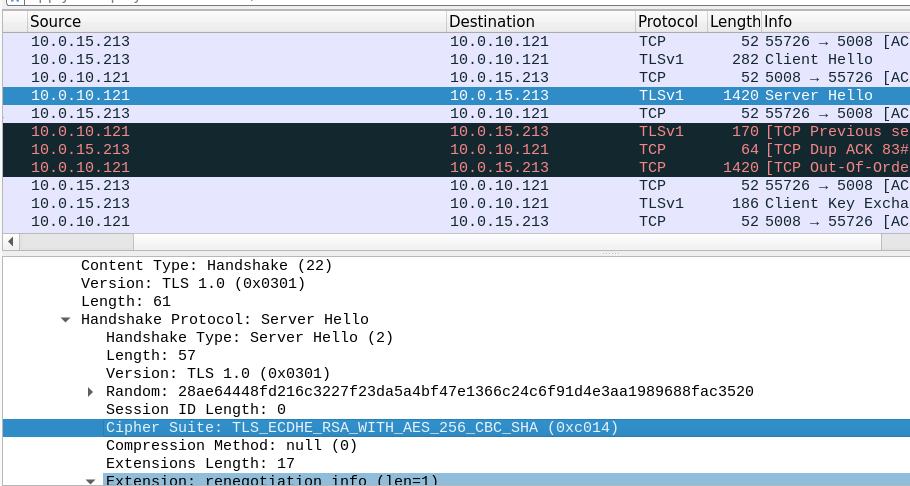
\includegraphics[keepaspectratio, width=\linewidth]{./figures/tls-handshake-cipher-spec.png}
    \caption{Negotiation on the cipher suite}
\end{figure}

Based on this, a scanner could change the list of cipher suites to enumerate all
cipher suites that the server will accept.

The server is vulnerable to BEAST attacks if it accepts TLS 1.0 handshake and support
cipher suites with CBC modes.

\begin{lstlisting}[language=bash]
python scan.py host port
\end{lstlisting}

The \texttt{openssl} utility is able to start a TLS server with many options.

\begin{lstlisting}
openssl s_server \
    -CAfile ca_cert.pem \
    -cert server_cert.pem \
    -key server_key.pem \
    -HTTP -port 5008 -tls1
\end{lstlisting}

\begin{figure}[htb]
       \centering
       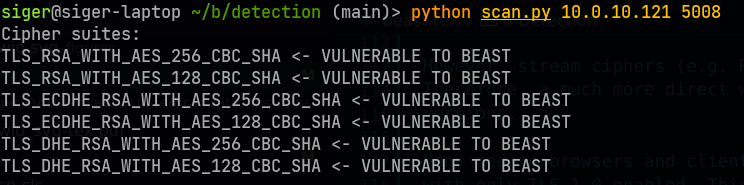
\includegraphics[keepaspectratio, width=\linewidth]{./figures/detection-output.png}
       \caption{Detection output on a TLS 1.0 server}
\end{figure}

% \subsection{}
%ACKNOWLEDGMENTS are optional
% The following two commands are all you need in the
% initial runs of your .tex file to
% produce the bibliography for the citations in your paper.
\bibliographystyle{abbrv}
\bibliography{beast}  % sigproc.bib is the name of the Bibliography in this case
% You must have a proper ".bib" file
%  and remember to run:
% latex bibtex latex latex
% to resolve all references
%
% ACM needs 'a single self-contained file'!
%
%APPENDICES are optional
\balancecolumns
\appendix
%Appendix A
% \section{Headings in Appendices}
% \section{Detection script for BEAST}
% \begin{lstlisting}[language=Python]
% \end{lstlisting}
\balancecolumns
\end{document}
